\documentclass[12pt]{report}
\usepackage{graphicx} % Required for inserting images
\linespread{1.2}

\usepackage[dvipsnames]{xcolor}
\usepackage{tikz}
\usepackage[breakable]{tcolorbox}
\appto{\bibsetup}{\raggedright}

\tikzstyle{mybox} = [draw=NavyBlue, fill=NavyBlue!5, ultra thick, rectangle, rounded corners, inner sep=10pt, inner ysep=15pt, text width=0.90\textwidth, align=left] 
\tikzstyle{boxtitle} = [fill=NavyBlue, text=white, ultra thick, rectangle, rounded corners, inner sep=10pt, inner ysep=8pt, text width=0.90\textwidth]

\newcommand{\BoxDef}[2]{%
\vspace*{10px}
\noindent

\begin{center}
\begin{tikzpicture}
    \node[mybox](box){\rule{0pt}{30pt}\ignorespaces#2\unskip};
    \node[boxtitle, anchor=north west] at (box.north west) {\textbf{#1}};
\end{tikzpicture}
\end{center}
}

\usepackage[]{hyperref}
\usepackage{amsmath}
\usepackage{amssymb}
\usepackage{bm}
\usepackage[top=2.5cm, bottom=2.5cm, left=3cm, right=3cm, centering]{geometry}
\usepackage{algorithm}
\usepackage{algpseudocode}
\usepackage{tabularx}
\usepackage{tabularray}
\usepackage{svg}
\usepackage{enumitem}
\usepackage{titlesec}

\begin{document}

\begin{titlepage}
\hrule
\vspace{15pt}
\begin{center}
    \Huge{\textbf{\Huge \textbf{Geospatial Analytics 24-25}} \\ Notes}\\
\end{center}
\vspace{15pt}
\hrule
\vfill
\hrule
\begin{center}
    \Large University of Pisa \\ M.Sc. in Data Science and Business Informatics
\end{center}
\end{titlepage}

\tableofcontents

\chapter{Introduction}

A geographic information system (GIS) is a computer system used to capture, store, query, analyze, and display geospatial data. \textbf{Geospatial data} describes both the location and the characteristics of spatial features: for example, if we want to describe a road, we may refer to its location and its features (length, name, speed limit, etc.). Other than single entities, geospatial data can also describe trajectories, specifying the sequence of locations constituting it.\\
The following chapter will give an overview of the basic concepts used in GISs and spatial data analysis.

\section{Geographic Coordinate Systems}

When using a GIS, any map layers used together must align spatially; to make sure this is true, we need to use some common spatial reference system for all maps. GIS users normally work with locations expressed on a plane using a coordinate system expressed in x- and y-coordinates, while the actual, real-life locations represented by them are on Earth's surface (which is ellipsoidal). A \textbf{map projection} is used to convert the Earth's surface to a plane.

The system used to locate points on Earth is called \textbf{geographic coordinate system}. This system is defined by two coordinates: \textbf{longitude} and \textbf{latitude}. They are angular measures which measure the angle at which the point can be found with respect to the \textbf{prime meridian} and the \textbf{equator}; longitute represents the angle east or west from the prime meridian, while latitude represents the angle north or south of the equatorial plane.

\textbf{Meridians} are lines of equal longitude. The prime meridian passes through Greenwich, England, and corresponds to 0°. \textbf{Parallels} are lines of equal latitude. The equator is the line corresponding to 0° latitude.

In a \textbf{plane coordinates} system, longitute and latitude correspond to x and y coordinates respectively. Logitude takes positive values in the easter hemisphere, and negative values in the western hemisphere; latitude takes positive values north of the equator, and negative values south of the equator.
\begin{figure}[!ht]
    \centering
    \includesvg[width=1.0\textwidth]{img/lat_lon_earth.svg}
    \caption{Latitude and longitude.}
    \label{fig:lat-lon-earth}
\end{figure}
\\
Longitute and latitude values may be expressed in different ways:
\begin{itemize}
    \item \textbf{Decimal degrees} (\textbf{DD}): represented by a single decimal value;
    \item \textbf{Degrees-minutes-seconds} (\textbf{DMS}): represented by a set of three values, corresponding to degrees, minutes, and seconds. 1 degree corresponds to 60 minutes, and 1 minute corresponds to 60 seconds;
    \item \textbf{Radians} (\textbf{rad}): similar to DD, but expressed in radians instead of decimal values: 1 degree is equal to 0.01745 rad.
\end{itemize}

As mentioned before, planet Earth can be approximated as an \textbf{ellipsoid}: this shape is obtained by rotating an ellipse by its shortest axis. Indeed, Earth is wider along the equator (its major axis) than it is between the poles (its minor axis). Another parameter that describes an ellipsoid is the \textbf{flattening} ($f$), calculated as $f = \frac{maj - min}{maj}$, and it describes the difference between the two axes.

A \textbf{datum} is a mathematical model of the Earth which is used as the reference to calculate the geographic coordinates of a point (or even the elevation, if we consider vertical datums). A datum is defined as: the pair \textit{longitude, latitude} of coordinates of an initial point wich will be the origin, an ellipsoid, and the separation of the ellipsiod and the Earth at the origin.

Distances on the Earth's surface are not straight lines; they are instead represented by \textbf{geodesics}: through any two points (not antipodal), there is exactly one ``great circle'' that connects them. The two points separate the great circle in two parts: the shorter of the two is their geodesic distance. Since the Earth is nearly spherical, geodesic distances are correct with an error up to $0.5\%$. The geodesic distance between points $A$ and $B$ is calculated using the \textbf{spherical law of cosines}:
\begin{equation*}
    \cos(d) = \sin(\textit{lat}_A) \sin(\textit{lat}_B) + \cos(\textit{lat}_B) + cos(\textit{lon}_A - \textit{lon}_B),
\end{equation*}
where $d$ is the angular distance between the two points. To convert $d$ to a linear distance measure, it can be multiplied by 111.32 km, which is the length of 1 degree at the equator. This formula is the basis from which the \textbf{haversine formula} is derived.

\section{Trajectories, Tessellations, Flows}

Let $u$ be an individual. A \textbf{trajectory} $T_u = \langle p_1, p_2, \dots, p_{nu} \rangle$ is a time-ordered sequence composed by the spatio-temporal points visited by $u$. A spatio-temporal \textbf{point} is a pair $p = (t,l)$, where $t$ is the time, and $l=(x,y)$ is the point visited at that time.

Given an area $A$, a \textbf{tessellation} is a set of geographical polygons with the following properties:
\begin{itemize}
    \item It contains a finite number of polygons called \textbf{tiles}:
    \begin{equation*}
        \mathbb{G} = \{g_i : i = 1, \dots, n\}
    \end{equation*}
    \item The tiles are non overlapping:
    \begin{equation*}
        g_i \cap g_j = \emptyset \,, \forall i \neq j
    \end{equation*}
    \item The union of all tiles completely covers the tessellation:
    \begin{equation*}
        \bigcup_{i=1}^n g_i = A
    \end{equation*}
\end{itemize}
A tessellation can be \textbf{regular} or \textbf{irregular} depending on the shape of its tiles. Regular tessellation may use equilateral triangles, squares, hexagons; irregular tessellation may use buildings, census cells, administrative units. A \textbf{spatial join} is used to associate a point with the tile it belongs to. Since the tiles are non overlapping and cover the entire area, each point belongs to one and only one tile. \textbf{Voronoi tesselations} are a particular type of tessellation that partition the plane into regions (called \textbf{cells}), each closer to a secific point (called \textbf{seed}) out of a set. Each of these cells is defined as the set of points that are closest to the seed of the cell itself than any other seed in that area.

Given a tessellation, the \textbf{flow}
\begin{equation*}
    y(g_i. g_j)
\end{equation*}
represents the number of people/objects moving between $g_i$ and $g_j$. A trajectory refers to a single entity, while a flow refers to the total amount of entities moving between two points. Flows can be derived from a set of trajectories, but the inverse is not true.

\section{Raster and Vector Data Models}

The raster and vector data models are two ways to represent geographic information in GISs. In both cases, data can be stored in several \textbf{thematic layers}, each of which contains a set of objects of the same nature. For example, a layer may contain information about buildings, another about streets, another about rivers, and so on.

The \textbf{raster data} model divides the space into a regular grid of square cells with a given size (which defines the \textbf{resolution}). This format is often used for images, where each element corresponds to a pixel. Depending on how much information is assigned to a cell, data can be \textbf{single-band} (one attribute per cell), or \textbf{multi-band} (several attributes per cell). Raster data is typically sourced from satellites.

The \textbf{vector data} model uses discrete objects (points, lines, polygons) to represent spatial features. Each object can have its own properties and relationship with the others. A \textbf{point} is a zero-dimensional object with a \textit{location} property (expressed as x,y coordinates). A \textbf{line} in a one-dimensional object with two properties: \textit{location} and \textit{lenght}. It be either straight or curved. A \textbf{polygon} is a two-dimensional object with three properties: \textit{location}, \textit{area}, and \textit{perimeter}. These objects are expressed differently depending on the data format used by the software/platform.

Objects in a layer are sometimes also called \textit{spatial features}; for this reasin, the variables associated to them are called \textit{attributes} (and not features). To represent geometric objects in a GIS, we can use one of the following models:
\begin{itemize}
    \item \textbf{Geo-relational data model}, where objects and attributes are stored separately, and associating each object to the corresponding attributes requires a join operation (at the advantage of possibly saving space if a certain attribute(s) is (are) only possessed by few objects);
    \item \textbf{Object-relational data model}, where objects and attributes are stored together in a single table, making retrieval much faster (but possibly increasing the amount of space needed to store everything). 
\end{itemize}

In principle, vectors can model everything; raster data is a discretized view of the same information. Raster data is better suited for ``dense'' data; it can be more efficient in those cases where a raster representation may need a very high number of objects, but precision is not a concern. Vector data can also be converted to raster data, and vice versa. \textbf{Rasterization} is the process of transforming vector data into raster data, and produces a discrete approximation. \textbf{Vectorization} is the inverse process: it may be difficult at times, and many algorithms and methods have been developed to perform it.

At times, vectors and raster information can be used together in multi-layer data. Some information is better modeled with one format than the other: for example, street networks or locations of interest are often encoded as vector layers, while things like land usage are encoded as raster layers.

\section{Spatial Operations}

The most important spatial operations are:
\begin{itemize}
    \item \textbf{Intersection}: returns all the points in common with the operands.
    \item \textbf{Union}: returns the union of the two operands. In some tools, They are kept as separate objects, meaning that the result is always a multipolygon. As an alternate operation, the same tools offer the \textbf{dissolve} operation, which instead merges the two objects into a single one.
    \item \textbf{Difference}: returns all the points in the first operand which are not in the second.
    \item \textbf{Buffering}: creates a buffer, i.e., an expanded area, around the object. The result is equivalent to replacing each point in the geometry with a circle with a given radius.
    \item \textbf{Spatial join}: like in relational databases, joins merge the information of two objects. THe join can be \textbf{inner} (the output contains only pairs in common with both objects), or \textbf{outer/left/right} (the output also contains non matching objects with the \textit{NULL} value in place of the missing attributes). 
\end{itemize}

\section{Spatial Patterns and Spatial Correlation}

\textbf{Point Pattern Analysi}s (\textbf{PAA}) is the study of point patterns, i.e., the spatial distribution of points in an area. Spatial distributions are typically categorized into three types:
\begin{itemize}
    \item \textbf{Uniform (discrete)}: points are evenly distributed in the area;
    \item \textbf{Random}: points are distributed according to a random process;
    \item \textbf{Clustered}: points appear to be grouped (clustered) in some areas.
\end{itemize}
A basic form of point pattern analysis consists in determining summary statistics such as mean center, standard distance, and standard deviational ellipse. \\
\textbf{Mean center} is the average of the x and y coordinate values:
\begin{equation*}
    \bar{s} = \left( \frac{\sum_{i=1}^n x_i}{n} , \frac{\sum_{i=1}^n y_i}{n} \right)
\end{equation*}
\textbf{Standard distance} measures the variance between the average distance of the features to the mean center:
\begin{equation*}
    d = \sqrt{\frac{\sum_{i=1}^n (x_i - \mu_x)^2 + (y_i - \mu_y)^2}{n}}
\end{equation*}
Similar to standand distance, \textbf{standard deviational ellipse} measures the standard distances for each axis:
\begin{align*}
    &d_x = \sqrt{\frac{\sum_{i=1}^n (x_i - \mu_x)^2}{n}} \\
    &d_y = \sqrt{\frac{\sum_{i=1}^n (y_i - \mu_y)^2}{n}}
\end{align*}

\textbf{Average Nearest Neighbor} (\textbf{ANN}) is an algorithm that can be used to study patterns. For each point, its nearest neighbor is found as the point with the smallest distance to it. The average of all points' nearest neighbor distance is calculated as $d_{obs}$, and normalized with regards to the expected average if the pattern were random ($d_{exp}$), obtaining a ratio:
\begin{equation*}
    R = \frac{d_{obs}}{d_{exp}}
\end{equation*}
If $R = 1$, the pattern is random. If $R < 1$, the pattern is clustered, because the distances are smaller than expected; if $R > 1$, the pattern is uniform (or at least more dispersed than random).

\textbf{Ripley's K-function} is another popular method for analyzing point patterns. Usually, its normalized version, called \textbf{L function}, is used. Given $n$ points in an area of size $A$, and a distance $d$, the L function is calculated as follows:
\begin{enumerate}
    \item Compute all $n*(n-1)$ distances between each pair of points;
    \item Compute $\phi$, the fraction of distances that are $ \leq d$;
    \item Compute
    \begin{equation*}
        L(d) = \sqrt{\frac{A}{\pi} \phi} \,.
    \end{equation*}
\end{enumerate}
$L(d) = d$ for random distributions. If $L(d)$ is higher, the data is more clustered; if it is lower, the data is more dispersed. Different values of $d$ can be explored to understand patterns at different spatial granularities.

Another important aspect is \textbf{density based analysis}. Density measurements can be either global or local. \textbf{Global density} is simply calculated as the ratio of observed points and the study region's area:
\begin{equation*}
    \hat{\lambda} = \frac{n}{A}
\end{equation*}
Density can also be measured at different locations of the study region. \textbf{Local density} is computed over a single tessellation cell; the chosen resolution will affect the resulting density calculation. \textbf{Kernel density} is another method of calculating density per-cell which considers also the points found in its neighborhood. Usually, given a cell $c$, the 8 adjacent cells are considered as the neighborhood $N_c$, and so the kernel density becomes:
\begin{equation*}
    \textit{Kernel density} \ (c) = \hat{\lambda}(c \cup N_c)
\end{equation*}
A variant is \textbf{weighted kernel density}, which assigns to each point a weight inversely proportional to the distance from the cell's center. Different weight functions can be used; a common one is the Gaussian function.

Autocorrelation is the correlation of the values of a same variable measured at different points in time (\textbf{temporal autocorrelation})/space (\textbf{spatial autocorrelation}). An example of spatial autocorralation may be checking how much the temperature values in the points of a layer are influenced by the neighboring values. According to \href{https://en.wikipedia.org/wiki/Tobler%27s_first_law_of_geography}{\textbf{Tobler's first law of geography}}, ``everything is related to everything else, but near things are more related than distant things'': this is the fundamental assumption in spatial analysis.

Popular measures of spatial autocorrelation are:    
\begin{itemize}
    \item \textbf{Moran's I}, which calculates the autocorrelation between values of each point against all other points in its neighborhood:
    \begin{equation*}
        I = \frac{\sum_{i=1}^n \sum_{j: x_j \in N_{x_i}} w_{ij} (x_i - \mu_x)(x_j - \mu_x)}{s^2 \sum_{i=1}^n \sum_{j: x_j \in N_{x_i}} w_{ij}} 
    \end{equation*}
    where $s^2$ is the variance of the $x$ values, and $w_{ij}$ is a weight, typically defined as the inverse of the distance between the two points. Positive values mean positive correlation, negative values mean negative correlation;
    \item \textbf{Geary's C}:
    \begin{equation*}
        C = \frac{n-1 \sum_{i=1}^n \sum_{j: x_j \in N_{x_i}} w_{ij} (x_i - x_j)^2}{2 (\sum_{i=1}^n \sum_{j: x_j \in N_{x_i}} w_{ij}) * \sum_{i=1}^n (x_i - \mu_x)^2}
    \end{equation*}
    The higher it is, the more different are nearby values (less correlation), the lower it is the closer they are (more correlation).
\end{itemize}
Both measures can also be interpreted as the average of local I/C values calculated across neighborhoods. These local values can be studied individually as well.

\section{Spatial Interpolation}

Spatial interpolation refers to the process of using points with known values (called \textbf{control points}) to estimate values at others. For example, we could estimate the temperature at a point with no recorded data by approximating it from known temperatures at nearby points. Ideally, control points should be well distributed across the study area, although this situation is rare in real-world applications since a study area oftentimes also contains data-poor areas.

Interpolation methods can be divided in two groups: \textbf{deterministic} and \textbf{stochastic}. The first group assumes that the known values are exact, with no assessment of errors for predicted values. The second group considers the presence of some random error in the known data and offers some assessment of prediction error with an estimated variance.
\begin{figure}[!ht]
    \centering
    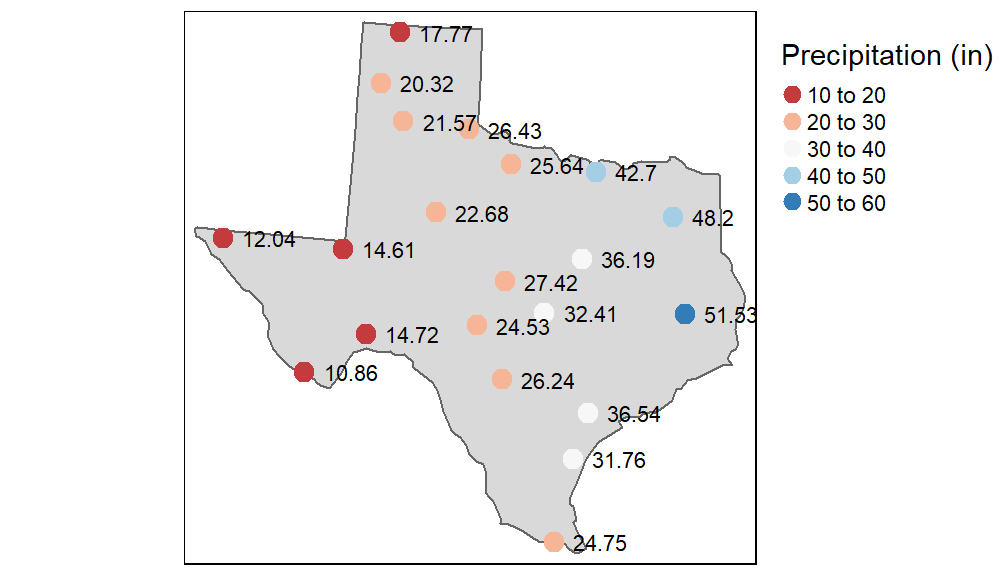
\includegraphics[width=0.5\textwidth]{img/interpolation_original.png}
    \caption{An example of samples corresponding to yearly precipitation recorded in different sites in Texas.}
    \label{fig:interpolation_original}
\end{figure}

\subsection{Deterministic Methods}

\subsubsection{Proximity Interpolation}

Proximity interpolation (also known as \textbf{Thiessen interpolation}) is one of the simplest and oldest interpolation methods. The goal is to assign to all unsampled locations the value of the closest sampled location, producing a Voronoi tessellation over the study area. All the points within the same cell have the same value. A problem of this approach is that surface values change abruptly across the perimeter of adjacent cells, which is not realistic.

\subsubsection{Inverse Distance Weighted Interpolation}

Inverse Distance Weighted (IDW) interpolation calculates an average value using nearby weighted locations. The weight of each sample location is inversely proportional to the distance; the value at location $j$ is given by:
\begin{equation*}
    \hat{Z}_j = \frac{\sum_i Z_i / d_{ij}^n}{\sum_i 1 / d_{ij}^n}
\end{equation*}
Here, $d_{ij}$ is the distance between points $i$ and $j$, and $n$ is an hyperparameter that controls the irrelevance of a point as the distance increases/decreases: the larger $n$ is, the less far away samples influence the interpolated value. For $n \rightarrow \infty$, the result is equivalent to proximity interpolation. \\
Values returned by this method are always within the range of the known values: $[Z_{min}, Z_{max}]$.

\begin{figure}[ht!]
    \centering
    \begin{minipage}{0.49\textwidth}
        \centering
        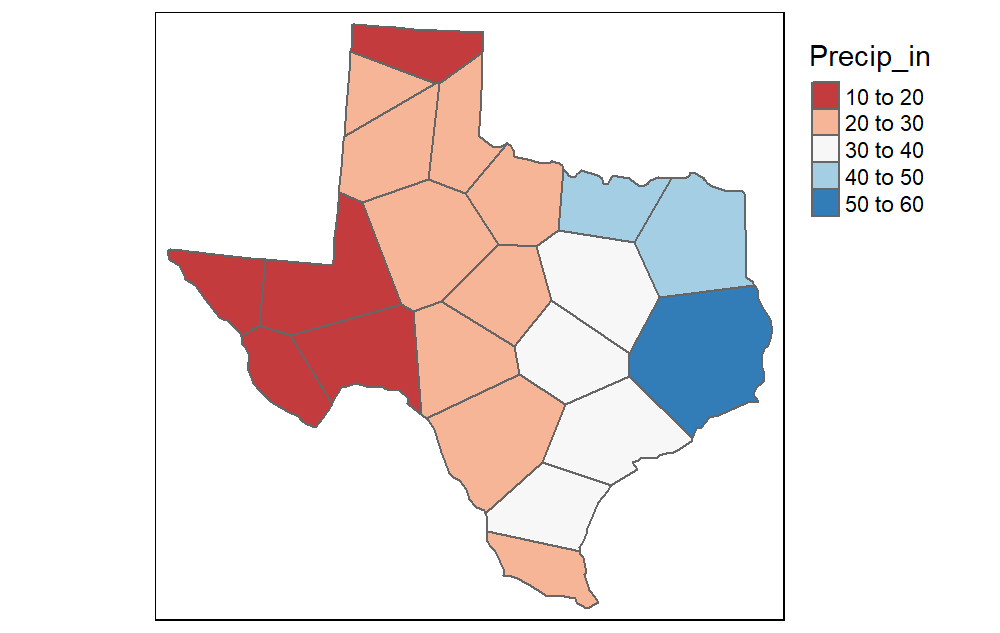
\includegraphics[width=\textwidth]{img/interpolation_proximity.png}
        \caption{Interpolated values obtained by proximity interpolation.}
        \label{fig:interpolation_proximity}
    \end{minipage}
    \hfill
    \begin{minipage}{0.49\textwidth}
        \centering
        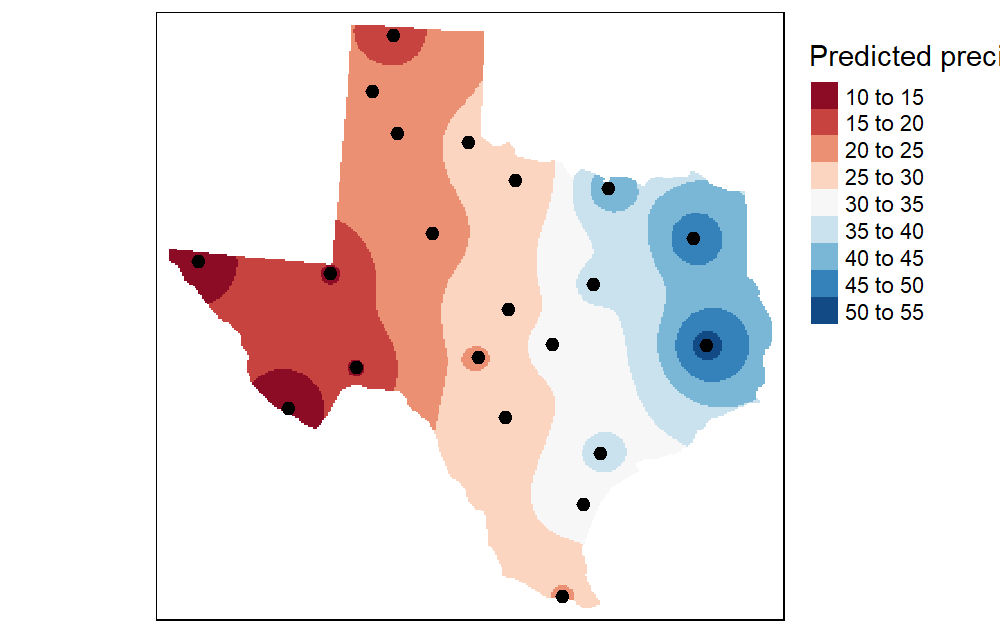
\includegraphics[width=\textwidth]{img/interpolation_idw.png}
        \caption{Interpolated values obtained by IDW interpolation.}
        \label{fig:interpolation_idw}
    \end{minipage}
\end{figure}

\subsection{Stochastic Methods}

\subsubsection{Trend Surface Interpolation}

Trend surface analysis approximates points with known values using a polynomial equation. The same equation can then be used to predict values at other points. Depending on the order of the polynomial, the approximation can be more or less complex:
\begin{itemize}
    \item A $0^{th}$ order surface is described by $Z = z$, where $c$ is the average value of all samples;
    \item A $1^{st}$ order surface is described by $Z = aX + bY + z$, where $X, Y$ are the coordinate pairs and $c$ is a constant;
    \item A $2^{nd}$ order surface is described by $Z = aX^2 + bY^2 + cXY + dX + eY + z$;
\end{itemize}
and so on. Changing the order allows the model to better capture the complexity of the data, but using a value that is too high may result in overfitting the data, meaning that the model is too dependant on the known information and does not provide a useful prediction.
\begin{figure}[!ht]
    \centering
    \begin{minipage}{0.49\textwidth}
        \centering
        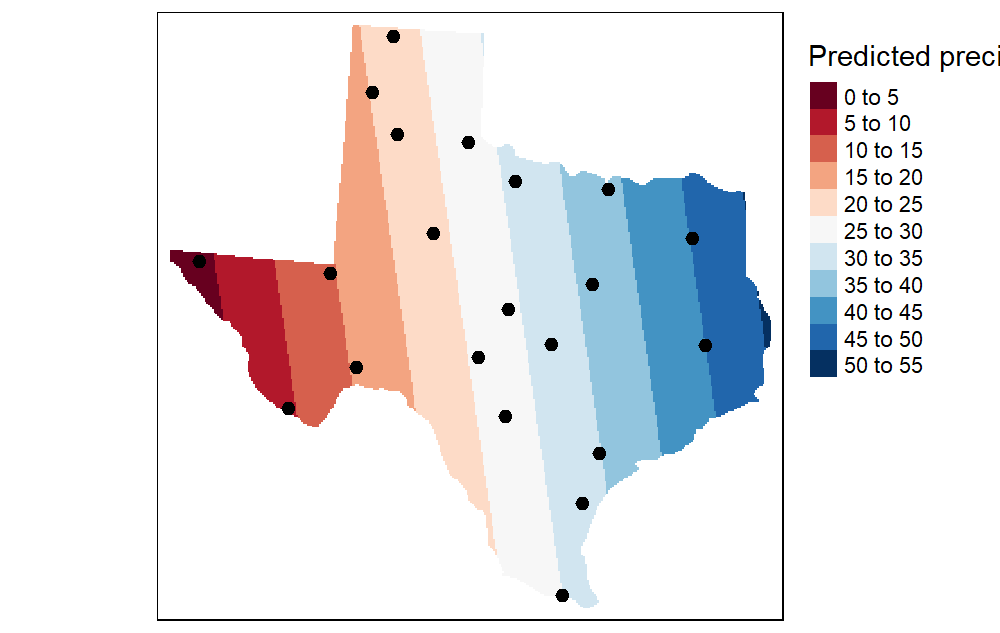
\includegraphics[width=\textwidth]{img/interpolation_fst_order.png}
        \caption{Interpolated values obtained by a $1^{st}$ order trend surface. The model is too rigid.}
        \label{fig:interpolation_fst_order}
    \end{minipage}
    \hfill
    \begin{minipage}{0.49\textwidth}
        \centering
        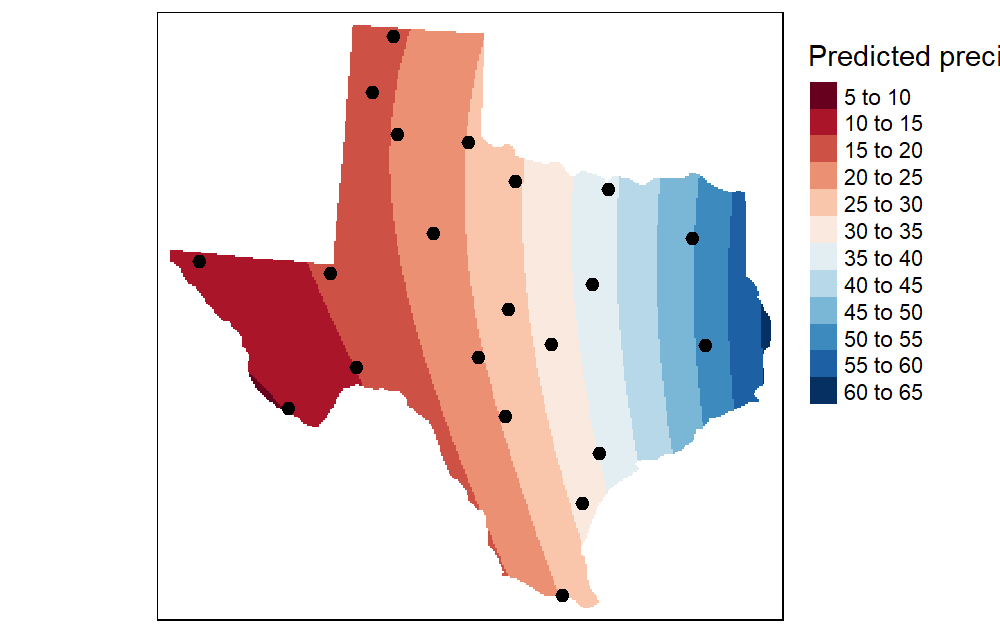
\includegraphics[width=\textwidth]{img/interpolation_snd_order.png}
        \caption{Interpolated values obtained by a $2^{nd}$ order trend surface. The model is better than before, but still not a good fit.}
        \label{fig:interpolation_snd_order}
    \end{minipage}
\end{figure}

\subsubsection{Kriging}

Kriging differs from other methods in that it can assess the quality of prediction with estimated prediction errors. It assumes that the spatial variation of an attribute is neither random nor deterministic; instead, it is a combination of some spatially correlated component, a ``drift'' (assumed for now to be null), and a random error term.

The first step is \textbf{de-trending the data}, so that mean and variance of the data are constant across the whole study area. This can be done by using any trend model and subtracting the predictions from the data. From this point on, the method will focus on residuals, i.e., the remaining variability in te data that is not explained by the global trend. The second step is \textbf{constructing a (semi)variogram}. For each pair of points $i$ and $j$, their semivariance is calculated as:
\begin{equation*}
    \gamma = \frac{(Z_i - Z_j)^2}{2}
\end{equation*}
The variogram is obtained as the plot of all the semivariances, using the $x$ axis to represent distances, and the $y$ axis to represent the semivariances. Usually, it is simplified by binning over the distance values and averaging the semivariances within each bin, obtaining a \textbf{sample experimental variogram}. The third step is to fit an \textbf{experimental variogram model} to find the parameters that best describe the spatial variance; there are many model variants, with the main ones being the Gaussian, linear, and spherical ones. Finally, \textbf{interpolation} can be performed. The general equation for estimating the residual at a point $j$ is:
\begin{equation*}
    z_j = \sum_{i=1}^s z_i W_i
\end{equation*}
where $s$ is the number of sample points used in the estimation, and $W_i$ is the weight assigned to point $i$. These weights are derived by solving a set of simultaneous equations.
\begin{figure}[!ht]
    \centering
    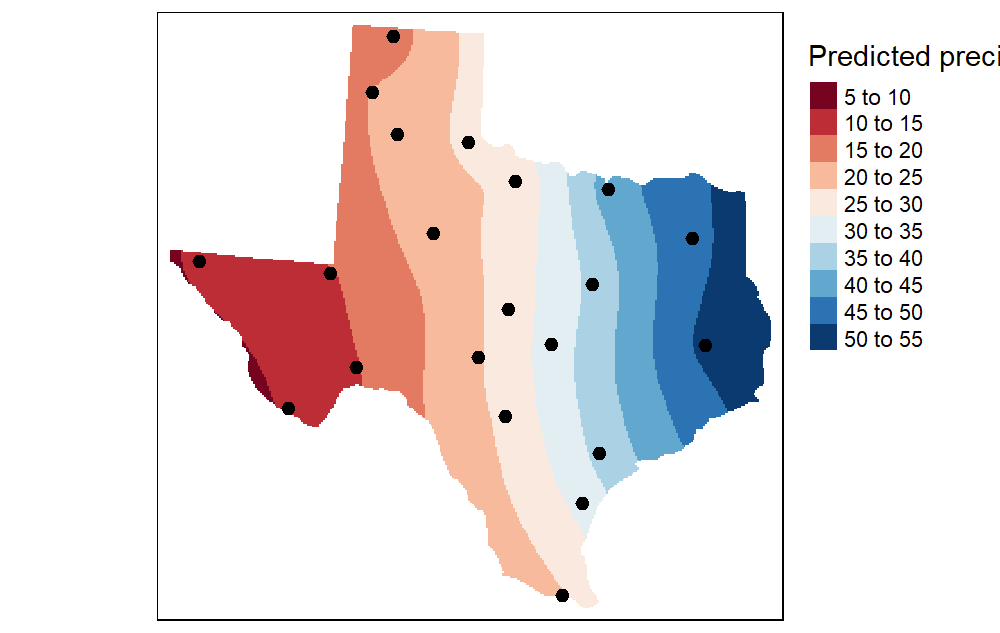
\includegraphics[width=0.5\textwidth]{img/interpolation_kriging.png}
    \caption{Interpolated values obtained by kriging.}
    \label{fig:interpolation_kriging}
\end{figure}

\subsection{Spatial Regression}

Regression has the goal of modeling the relationship between a target variable and a (set of) independent variable(s). The difference with interpolation is that in the latter, only the target variable data and the spatial coordinates are used, while in regression there is information about other non-spatial attributes to make predictions.

Spatial regression extends the typical regression method to include information about a point's neighborhood:
\begin{equation*}
    (P_i) = \underbrace{\alpha + \beta X_i + \epsilon_i}_{\parbox{7.5em}{\scriptsize\centering Standard regression model}} + \underbrace{\delta \sum_j w_{ij} X_j}_{\parbox{7.5em}{\scriptsize\centering Summary information about neighbors}}
\end{equation*}

\section{Co-location Pattern Mining}

Co-location pattern mining is the process of finding subsets of spatial features whose instances are frequently located together in space. It is similar to traditional frequent itemset mining, although defining ``transactions'' is not as immediate, since there is no explicit way to isolate instances into groups.

Given:
\begin{itemize}
    \item A set of features $F = \{f_1, \dots, f_m\}$;
    \item A set of instances $O = \{o_1, \dots, o_n\}$;
    \item A neighbor relation $R$ between pairs of instances, s.t. $R(o_1, o_2) \iff d(o_1, o_2) < \textit{thresh.}$; 
\end{itemize}
a \textbf{co-location pattern} $CL = \{f_1, \dots, f_k\} \subseteq F$ is a subset of features, and an \textbf{instance of a pattern} $I = \{o_1, \dots, o_k\} \subseteq O$ is a subset of objects s.t.:
\begin{itemize}
    \item For each $f \in F$, there is exactly one object $o \in O$ of type $f$, anc vice versa;
    \item $I$ forms a clique w.r.t. $R$ (i.e., all pairs of objects are connected to each other).
\end{itemize}
A co-location pattern that contains $k$ spatial features is called size-$k$ co-location pattern.

To measure the prevalence of a given pattern, we use two measures; the \textbf{participation ratio} (of a feature within a pattern):
\begin{equation*}
    PR(CL, f_i) = \frac{\#|\pi_{f_i} (\textit{instances(CL)})|}{\#|\textit{instances(CL)}|}
\end{equation*}
and the \textbf{participation index} (of the entire pattern):
\begin{equation*}
    PI(CL) = \min_{i=1}^k PR(CL, f_i)
\end{equation*}
A co-location pattern is called \textbf{prevalent} if its partecipation index is greater or equal than a given threshold \textit{minprev}. The participation index is anti-monotone, which means that the participation index of a co-location pattern is always lower or equal to that of its sub-patterns.

\section{Trend Detection}

Spatial trend analysis is the process of finding patterns of change of non-spatial attributes in the neighborhood of some object in the study area. It is analogous to trend analysis in time series, but applied to spatial data, where the linear direction of time is replaced by the many possible paths that can be formed in space. The most notable paths of interest usually start from a common location (e.g., a city center), have meaningful shape, and show a statistically significant trend.

Let $g$ be the neighborhood graph that represents all the neighborhood relationships among objects in the study area. Let $o$ be one such object, which is considered the starting point of paths. Let $a$ be a subset of all non-spatial attributes, in which paths must be found in. Let $t$ be a type of function (e.g., linear, exponential) used for regression. Then, the goal of spatial trend detection is to discover the set of all neighborhood paths in $g$, starting from $o$, having a trend of type $t$ in attributes $a$, with a correlation greater or equal to a given threshold \textit{minconf}.

To isolate these relevant paths, special filters are used to select subsets of all paths. There are many ways to define such filters; some examples are reported in Fig \ref{fig:trend_filters}.
\begin{figure}[!ht]
    \centering
    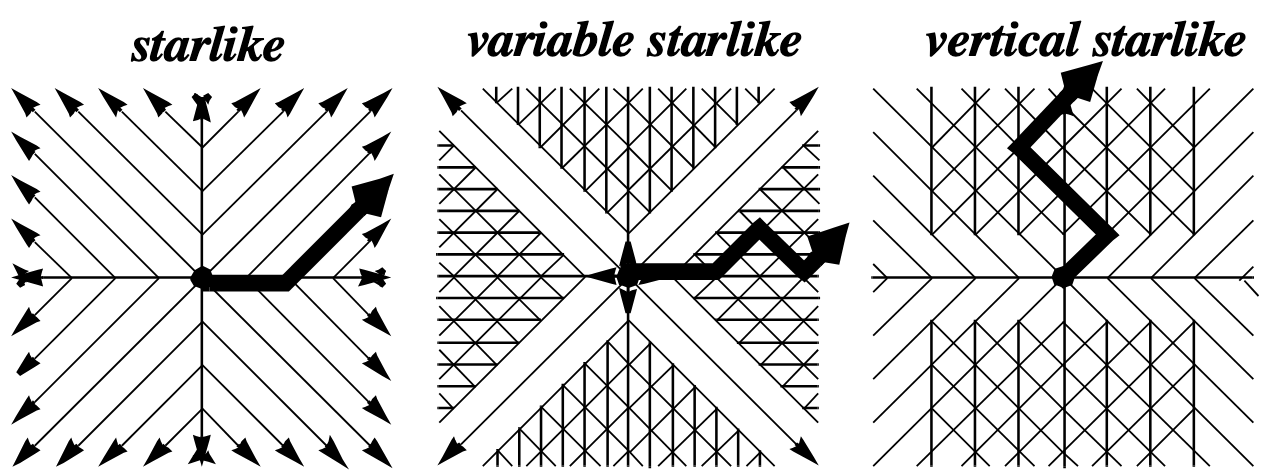
\includegraphics[width=0.75\textwidth]{img/trend_filters.png}
    \caption{Examples of possible filters. The \textit{stralike} filter allows paths that deviate in a specific diagonal direction; the \textit{variable starlike} filter allows paths that can deviate diagonally multiple times; the \textit{vertical starlike} filter restricts horizontal deviations in favor of vertical ones.}
    \label{fig:trend_filters}
\end{figure}
\chapter{Spatial and Mobility Data}

The study of human mobility data has a wide range of applications, such as urban planning, epidemic control, transportation management, immigration monitoring. The last decade has seen a rapid increase of digital traces that represent human movements. Examples of this data are those generated by GPS devices embedded in phones or cars, mobile phone records collected by telco companies, and geotagged social media posts. This chapter will describe the main characteristics of such data.

\section{GPS Data}

\textbf{Global Navigation Satellite Systems} (\textbf{GNSS}) use satellites to provide geo-spatial positioning of objects on the Earth's surface in terms of longitude, latitude, and altitude. There are currently multiple systems managed by different countries of the world. The most famous GNSS is the US \textbf{Global Positioning System} (\textbf{GPS}), and receivers are now embedded in many commonly used tools such as smartphones, cars, and wearable devices. 

GPS can be thought of a system of three main components: a space segment, a control segment, and a user segment. The \textbf{space segment} consist of a constellation of 24+ satellites orbiting around the planet, circling it twice a day in six equally spaced orbits. Each orbit has four satellites, and any user will always see at least four satellites from any point on Earth. The \textbf{control segment} consist of all the ground facilities used to track/command the satellites and monitor their transmissions. The \textbf{user segment} is represented by the GPS receivers in the user devices. On mobile phones, GPS receivers are activated by software that requires the user's position. On cars, receivers automatically turn on as the car starts. Signals are sent to a server every few seconds up to every few minutes; their precision can range from a few centimeters to meters, depending on the quality of the device.

To identify a point on Earth, a total of four satellites are used (three to identify the point, a fourth one for redundancy): each satellite broadcasts a radio signal at the speed of light that contains information about its location, status, and time of the on-board atomic clock. When the signal hits the device receiver, the time of arrival is compared to that of the send to calculate the distance $d$ from the satellite.

Using this distance, we can imagine a sphere of radius $d$ centered around the satellite. The intersection of all the spheres centered around the involved satellites is the exact location of the device. 
\\
The GPS traces format is as follows:
\begin{center}
$(u, lat, lng, alt, t)$
\end{center}
where:
\begin{itemize}[itemsep=-5pt, label=-]
    \item \textit{u} is the user/receiver ID;
    \item \textit{lat} is the latitude;
    \item \textit{lng} is the longitude;
    \item \textit{alt} is the altitude;
    \item \textit{t} is the timestamp.
\end{itemize}

\paragraph{Pros}
Ubiquitous, produces high resolution, dense traces.

\paragraph{Cons}
Rarely publicly available, no semantic information (e.g., what the user is doing, if he/she is in a building or outside), prone to errors when signal is noisy or absent, and small samples.

\section{Mobile Phone Records}

Mobile phone coverage reaches almost 100\% of the population of most countries. Telco companies collect the activity of phone users for billing purposes, storing information about where users are located, when they communicate with others, and who they communicate with. This type of information can be split in the following three groups.

\paragraph{Call Detail Records} CDR are generated each time a user makes/receives a call or an SMS. A CDR is a tuple
\begin{center}
$(n_o, n_i, t, A_o, A_i, d)$
\end{center}
where:
\begin{itemize}[itemsep=-5pt, label=-]
    \item $n_o$ is the caller's ID (can be the phone number, but it should be anonymized for privacy reasons);
    \item $n_i$ is the receiver's ID (same as above);
    \item $t$ is the timestamo if the call;
    \item $A_o$ is the ID of the antenna the caller is connected to;
    \item $A_i$ is the ID of the antenna the receiver is connected to;
    \item $d$ is the duration of the call.
\end{itemize}

\paragraph{eXtended Detail Records}
XDR are generated when a device uploads or downloads data from the Internet. These connections can be both human-triggered and device-triggered (e.g., software updates, background synchronization). An XDR is a tuple
\begin{center}
$(n, t, A, k)$
\end{center}
where:
\begin{itemize}[itemsep=-5pt, label=-]
    \item $n$ is the user's ID;
    \item $t$ is the timestamp of the connection;
    \item $A$ is the ID of the antenna the user is connected to;
    \item $k$ is the amount of KB of data transferred.
\end{itemize}

\paragraph{Control Plane Records}
CPR are used to check the status of the network, and are generated each time a device connects to a new antenna. These records are exclusively network-triggered. A CPR is a tuple
\begin{center}
    $(n, t, A, e_1, e_2, \dots, e_n)$
\end{center}
where
\begin{itemize}[itemsep=-5pt, label=-]
    \item $n$ is the user's ID;
    \item $t$ is the timestamp of the connection;
    \item $A$ is the ID of the antenna the user is connected to;
    \item $e_i$ are the ``events'' that happen in the network.
\end{itemize}

\paragraph{Pros}
Ubiquitous, huge sample size, rich and multidimensional (give information about space, time, and social connections among users, since we can know who calls/messages who).

\paragraph{Cons}
Not publicly available, much more sparse and low resolution than GPS, suffers from ping-pong effect (since areas of influence of antennas are not perfectly regular and may overlap, a device may rapidly flip between them).

\begin{figure}[!ht]
    \centering
    \includesvg[width=\textwidth]{img/mobile_data_comparison.svg}
    \caption{Comparison of densities of different data types.}
    \label{fig:mobile-data-comparison}
\end{figure}

\section{Location-based Social Networks}

Certain social media platforms allow users to geotag their posts, i.e., assign geographic and temporal information. This information can be represented by absolute data (latitude, longitude), relative data (distance from some point of interest), or symbolic (home, office, stadium, shopping mall).
This geospatial information can then be easily coupled with the social network structures of connected users, allowing us to consider the social dimension in our analysis. A LBSN record is a tuple
\begin{center}
    $(u, t, lid, lpos, post)$
\end{center}
where:
\begin{itemize}[itemsep=-5pt, label=-]
    \item $u$ is the user's ID;
    \item $t$ is the timestamp of the post;
    \item $lid$ is the location ID;
    \item $lpos$ is the location position;
    \item $post$ is the content of the text post.
\end{itemize}

\paragraph{Pros}
Ubiquitous, can provide precise information with little error, carries semantic information.

\paragraph{Cons}
Is very sparse (even more than mobile phone records), suffers from self-selection bias (users that frequently produce such content tend to belong to a specific demographic).

\section{Road Networks and Points of Interest}

\textbf{Road networks} describe streets and their intersections. They are usually represented by multigraphs, where a node is an intersection and an edge is a road. Nodes and edges are geometries, encoded as Point, Lines, or Polygons. A road network is described by a two sets of records: the first contains all the nodes, the second all the edges. A node record is a tuple
\begin{center}
    $(id, lat, lng, streets, geom)$
\end{center}
where:
\begin{itemize}[itemsep=-5pt, label=-]
    \item $id$ is the node ID;
    \item $lat, lng$ are the geographic coordinates;
    \item $streets$ number of streets crossing in that intersection;
    \item $geom$ is the geometric shape of the node (usually a Point).
\end{itemize}
An edge record is a tuple
\begin{center}
    $(id, u, v, f_1, \dots, f_k, geom)$
\end{center}
where:
\begin{itemize}[itemsep=-5pt, label=-]
    \item $id$ is the edge ID;
    \item $u$ is the origin node;
    \item $v$ is the destination node;
    \item $f_i, \dots, f_k$ are the road characteristics (e.g., if the road is one-way only, its length, number of lanes, name, speed limit);
    \item $geom$ is the geometric shape of the edge (usually a Line).
\end{itemize}
Road networks help associate GSP traces to actual streets, and can find routes between two places. These structuresa are also aften used in simulations for traffic management and urban planning.

\textbf{Points of interest} describe certain geospatial entities in a city, such as grocery stores, transit stops, restaurants, etc. They carry semantic information about activities in cities and associated human behaviour. A POI record is a tuple
\begin{center}
    $(id, f_1, \dots, f_n, geom)$
\end{center}
where:
\begin{itemize}[itemsep=-5pt, label=-]
    \item $id$ is the POI ID;
    \item $f_i, \dots, f_n$ are the POI characteristics (e.g., name, type of building, road nodes involved);
    \item $geom$ is the geometric shape of the POI (usually a Point or a Polygon).
\end{itemize}
\chapter{Data Preprocessing}

Data that represents trajectories of moving entities is often affected by errors. Their presence can greatly influence the result of analysis, so it is important to identify and remove them. Additionally, datasets tend to contain huge amounts of objects, meaning that the time and space complexity that may be too high. Finally, individual trajectories that are too long and complex may cause the failure of data mining algorithms due to the inability of extracting details from them. Summarizing the information carried by trajectories via a preprocessing phase is a necessary step to make sure subsequent analysis can be carried out efficiently and effectively.

Preprocessing techniques can be divided into two families: context-based filtering, and movement-based filtering. \textbf{Context-based filtering} relies on contextual geographical information provided by the environment, such as road networks, to remove points that are deemed to be errors. These methods may not always be effective, since they assume that trajectories must always be on a road (or adapt in some way to the available data); this may not always be true, for example for vehicles moving across the sea or open fields, or for pedestrians. \textbf{Movement-based filtering} uses only the geometry and dynamics of the movement described by the trajectory to find points that do not match the expected behaviour of the moving entity.

\section{Movement-based Filtering}

\subsection{Speed-based Filtering}

This filtering is based on the idea that the speed of the moving entity must always be within a certain range of allowed values, without any abrupt change. Initially, the first point of the trajectory is found and set as valid; then, each subsequent point is scanned in order according to the timestamp, and the speed $v$ between the current and the previous point is calculated:
\begin{itemize}
    \item If $v$ is larger than a given threshold, the point is marked as invalid and removed from the trajectory;
    \item If $v$ is within the threshold, the point is marked as valid and kept.
\end{itemize}

\begin{figure}[!ht]
    \centering
    \includesvg[width=0.70\textwidth]{img/filtering_speed.svg}
    \caption{Example of speed-based filtering: point \textit{e} is removed from the trajectory as it would imply a speed higher than the threshold.}
    \label{fig:filtering-speed}
\end{figure}

\section{Context-based Filtering}

\subsection{Point Map Matching}

Map matching is the procedure of determining which road on a map a vehicle is using, given a set of GPS points. This approach both filters out noise and outliers, and adds new information to the dataset by associating each point with an identifier of the road it is matched to. Once points have been mapped to a specific road, any point farther than a certain threshold can be removed as noise.

The main issues of this approaches are:
\begin{itemize}
    \item Projecting individual points requires a comparison for each point and each road segment, which can be computationally expensive;
    \item In some cases, the same point could be potentially assigned to multiple road segments, but limiting ourselves to consider the closest one may not always be the best choice;
    \item Matching points individually can lead to inconsistencies, especially when the road network is very dense.
\end{itemize}

\subsection{Route Reconstruction and Trajectory Map Matching}

\paragraph{Route Reconstruction}
Route reconstruction tries to infer the path taken by a moving entity by connecting the available points and possibly creating new ones; this technique is useful in cases where data is generally sparse or has large missing gaps. Usually, we assume the entity always takes the shortest (or best) path between two consecutive points; if an area allows free movement, the entity is assumed to move in a straight line. If there are limitations, such as the presence of buildings, the path must adapt to them. Since we often have attributes describing the characteristics of roads, the optimal path can be found by trying to maximize or minimize certain features: the total path duration in time, fuel consumption, $CO_2$ emissions, etc.

Common algorithms used for route reconstruction are \textbf{Dijkstra's minimum cost path algorithm}, which is efficient and can handle cycles, although it requires non-negative costs, and \textbf{Bellman-Ford's algorithm}, which is less efficient and can't handle cycles, but allows negative costs.

\paragraph{Trajectory map matching}
This is a more advanced version of point map matching that takes as input a whole trajectory (wheter it comes from raw data or from a reconstruction step), and adapts it to a road network considering spatial, temporal, and contextual constraints for the whole path. Common approaches are shortest-path based, and probability-based.

\textbf{Shortest-path based Map Matching} starts by matching only the first and last point of the path to the road segments, as in point map matching, and then finding the optimal path that connects them. A threshold is set as the maximum distance allowed between a segment and a GPS point for the two to be considered matching; using this threshold, \textbf{cutting points} are found. A cutting point can be of two types: the first type is the point that is the farthest from the current optimal path, and the second type are the points whose distance fall within the threshold. If a cutting point of the first type is found, the path is split in two, and a new optimal path that passes by that point is found. These steps run recursively on each half until all the points are reasonably close to the optimal path.

\textbf{Probability-based Map Matching} considers the probability that an entity may move from one road segment to another. State-of-the-art implementations use Hidden Markov Models to model the trajectory as a sequence of state transitions.

\section{Trajectory Simplification}

Many algorithms on trajectories tend to be very expensive, and their complexity is tied to the number of points in the dataset. Trajectory simplification is used to reduce the number of points without affecting the quality of results. Typical cases in which simplification can be used are for straight line movement (the entity keeps moving in a straight line, so the whole trajectory/subtrajectory can be represented as a single segment), or negligible movement (the entity stays still for some time, accumulating GPS traces in the same spot). Some standard methods for polygonal curve simplification include Ramer-Douglas-Peucker, and Driemel-HarPeled-Wenk.

\textbf{Ramer-Douglas-Peucker} is one of the most successful simplification algorithms, used in many fields other than GIS, such as computer vision and pattern recognition. A pseudocode of the algorithm is found below.
\begin{algorithm}
\caption{Ramer-Douglas-Peucker pseudocode.} 
\begin{algorithmic}[1]
    \Function{RamerDouglasPeucker}{$P, \varepsilon, p_i, p_j$} \Comment{$P = \langle p_1, \dots, p_n \rangle$}
    
    \State Find vertex $p_f \in \langle p_i, \dots, p_j \rangle$ farthest from the line $p_i p_j$.
        
    \State $\textit{dist} \gets$ distance between $p_f$ and $p_i p_j$.

    \If{$\textit{dist} < \varepsilon$}
        \State \Call{RamerDouglasPeucker}{$P,p_i,p_f$}
        \State \Call{RamerDouglasPeucker}{$P,p_f,p_j$}
    \EndIf

    \State Return line $p_i p_j$.
    \EndFunction
\end{algorithmic}
\end{algorithm} \\
The time complexity is $T(n) = O(n) + T(n-1) = O(n^2)$ in the worst case, but it is usually much faster in practice.
\begin{figure}[!ht]
    \centering
    \includesvg[width=0.80\textwidth]{img/RDP.svg}
    \caption{Example of one step Ramer-Douglas-Peucker simplification.}
    \label{fig:ramer-douglas-peucker}
\end{figure}


\textbf{Driemel-HarPeled-Wenk} is not recursive, unlike the previous, but instead simplifies the line starting from the very first point and iteratively removes points that fall within a certain radius from the current one, substituting all of them with a single line that goes from the current point to the first point in the trajectory more distant than that radius. The pseudocode is below.
\begin{algorithm}
\caption{Driemel-HarPeled-Wenk pseudocode.}
\begin{algorithmic}[1]
    \Function{DriemelHarPeledWenk}{$P, \varepsilon$} \Comment{$P = \langle p_1, \dots, p_n \rangle$}
    
    \State $P' \gets p_1$.
    \State $i \gets 1$.
    
    \While{$i \leq n$}
        \State $\textit{curr} \gets p_i$.
        \State $j \gets i+1$.
        \While{$\textit{dist}(p_i, p_j \leq \varepsilon)$}
            \State $j \gets j+1$.
            \If{$j > n$}
                \State $i \gets n$.
                \State Break. 
            \EndIf
        \EndWhile
        \State Add $p_j$ to $P'$.
    \EndWhile

    \State Return $P'$.
    \EndFunction
\end{algorithmic}
\end{algorithm}

Either way, simplification has the side effect of modifying average speed estimates, as simpler, straighter paths imply a slower average speed compared to more complex, chaotic ones.

\section{Stop Detection for Trajectory Segmentation}

GPS data is normally formed by a continuous stream of points, but there is no explicit separation between the trajectories of the same entity. \textbf{Stop detection} is a technique used to identify moments in which the entity is staying still (or moving very slowly) to be used as endpoints of different trajectories. For example, if we consider a person moving through a regular work day, we may observe that person move away from a spot (likely his/her house), then stop at what is either school or work, then make another stop at the gym, and finally return back home. Every movement between each of these stops can be isolated as its own trajectory.

The general criteria is: the estimated speed from a set of points is very low (i.e., very little movement over a long time interval), the set of points represent a stop. The sequence of points between stops is a trajectory. To check if a point belongs to a stop, typical space and time thresholds are $Th_S \in [50, 250]$ (meters), and $Th_T \in [1, 20]$ (minutes), but depending on the context, these values may change: thresholds for a car are different from those for a pedestrian, for example.

When it comes to vehicles specifically, stops can often be detected by simply checking when the engine is on or off. This is generally good, but may not detect stops that are very short. A more general approach is to use a density-based approach: the faster an entity is, the less of its own points are found around it as it is moving. 

After trajectory segmentation has been performed, we can use them to study the behaviour of the individual, and eventually find deviations from the norm. A way to represent this information is building the entity's \textbf{Individual Mobility Graph}, where each location is a node and each movement is an edge; this means that for each trajectory, only the starting and ending locations are recorded in the graph. Naturally, denser areas with more nodes will represent important places. These locations are identified using a clustering algorithm, and are each associated with their frequency; trips between points belonging to the same cluster (location) are then aggregated as edges between the entire clusters. The basic assumption is that the location with the highest frequency is home, the second most frequent location is work, and so on. An alternative approach also considers the actual time of the day the traces were recorded at: points recorded during nighttime or early morning are more likely to be home, while those recorded during the morning and early afternoon are more likely to be work.

Other than GPS, phone data can also be used to infer important locations. By analyzing the calls and messages sent or received by the user, we can identify what are called \textbf{personal anchor points}, which are the most frequently contacted antennas. These points can also be labeled as home/work by considering the time of the day the calls were made or received.

\section{Activity Labeling}

After locations have been identified, an ulterior step is to assign to each of them a specific activity the user carries out once it arrives there. The first step is to assign a location to a set of actual point of interest that are close by. The POIs are then also associated with an activity, for example: ``eating out'', ``shopping'', ``working'', ``education''. At the end, the available data will be:
\begin{itemize}[itemsep=-5pt, label=-]
    \item For each POI, the category, the opening hours, the location;
    \item For each trajectory, the stop location, the stop duration, the time of day;
    \item For each user, the max walking distance (as in, how far the person is likely to walk after parking).
\end{itemize}
Each POI is associated to a certain probability of being the reason for the stop, calculated as a function of the information above. Finally, a stop is annotated with the activities and relative probabilities of the POIs close by.



\chapter{Individual and collective human mobility}

Human mobility refers to the movement in space and time of human beings. Individual mobility is the movement of a single person, while collective mobility is the movement of a group of people. In this chapter, a few basic concepts about human mobility are introduced: the laws of individual human mobility, abd the techniques used to model it.

\section{Individual Human Mobility}

\section{Metrics}

\paragraph{Travel Distance (Jump Length)}

Travel distance is the distance between two consecutive locations visited by the individual. Travel distance may also be called in different ways depending on the context it is used in; the term ``jump length'' is is used to refer to different appearances of the same object in different locations, without necessarily implying a direct movement between them. An early example of mobility analysis involved information about the spatial trajectories of bank-notes. The data was sourced from a US-based website where users could input the identifier of their dollar bills, specifying where they are located. In this sense, the distance between two different locations in which a bank-note appears in is a jump length.

Regardless of how it is defined, distance, denoted as $\Delta r$, is calculated as
\begin{equation*}
    \Delta r = \| r(t) - r(t + dt) \|_2
\end{equation*}
i.e., the Euclidean distance between the locations recorded at intervals $t$ and $t + dt$. It is interesting to study the distribution of $\Delta r$ within a population, approximating the probability distribution function of distances/jump lengths, $P(\Delta r)$. Empirical studies observed how this distribution follows a \textit{power-law}: a scale-free distribution (i.e., with no/meaningless mean) with a heavy tail:
\begin{equation*}
    P(r) \sim r^{-(1+\beta)}
\end{equation*}
where $\beta$ is the scaling exponent, which is chosen depending on the context.
\begin{figure}[H]
    \centering  
    \includesvg[width=0.75\textwidth]{img/zipf.svg}
\end{figure}
Power law behaviour has been observed in the trajectories of mobile phone users as well, specifically following a truncated power law:
\begin{equation*}
    P(r) = (r + r_0)^{-\beta} \exp(-r/\kappa)
\end{equation*}
where $r_0$ and $\kappa$ are the cutoffs of smaller and larger values of $\Delta r$.

What this means is that there are a lot of individuals who tend to move short distances; as the distance increases, the number of individual sharply decreases. However, there are still a few individuals who move very long distances (the distribution is not exponential).

\paragraph{Radius of Gyration}
Humans tend to habitually move a characteristic distance away from their starting locations. This distance can be quantified by the radius of gyration, $r_g$, defined as the root mean square distance of a set of points:
\begin{equation*}
    r_g = \sqrt{\frac{\sum_{i=1}^{N} \| r_i - r_{\textit{cm}} \|^2}{N}}
\end{equation*}
where $r_i$ are the coordinates of the $N$ individual locations the person visited, and $r_{\text{cm}}$ is the center of mass of the set of points (their centroid):
\begin{equation}
    r_{\textit{cm}} = \frac{\sum_{i=1}^{N} r_i}{N} 
\end{equation}
It was observed that the distribution of the radii of gyration of a population of individuals also follows a truncated power law.
\begin{figure}[H]
    \centering
    \includesvg[width=0.75\textwidth]{img/rog.svg}
    \caption{Radii of gyration of two different individuals. The red circle indicates their house, while the blue circles are the locations they visited.}
\end{figure}
What can be observed from data is that people with a small radius of gyration tend to travel mostly over small distances, while those with a large radius tend to have a combination of a lot of short travels and a few long ones.

An interesting aspect to consider is the phenomenon of \textbf{saturation}, observed during the temporal evolution of $r_g$; the average $r_g$ of a person shows a logaritmic increase with time, which can be attributed to the fact that people tend to follow regular travel patterns and after a certain amount of time, they have visited all the places they usually go to, leading to a stable $r_g$.

By itself, the radius of gyration does not carry any information about the relevance of a certain location in an individual's movements. An individual who spends most of his/her time in his/her most visited locations (e.g., home and work) will have a large $r_g$ if the two are far away; if instead they are close to each other, the $r_g$ may still be large, since there are likely other longer movements that contribute to the radius of gyration. To address this issue, one can consider the frequency of visits to a location, ranking them accordingly, and then calculate the \textbf{$k$-radius of gyration}:
\begin{equation*}
    r_g^{(k)} = \sqrt{\frac{\sum_{j=1}^k n_j (r_j - r_{\textit{cm}^{(k)}})^2}{N_k}}
\end{equation*}
where $N_k$ is the number of visits to the $k$ most frequented locations, $r_{\text{cm}}^{(k)}$ is the centroid of those top $k$ locations, and $n_j$ is the number of visits to the $j^{\textit{th}}$ location. The frequency of visits also follows a power law distribution, since people will devote most of their time to few places (home, work, school, etc.), and less and less time to others.

The analysis of CDR and GPS traces revealed that there are two distinct groups of individuals: the \textit{k-returners}, whose radius of gyration is well approximated by their k-radius of gyration for $k \geq 2$, and the \textit{k-explorers}, whose k-radius is very small compared to their overall $r_g$.

\subsection{Predictability}
A way to represent the movements of an individual is by constructing its \textbf{individual mobility network}, i.e., a graph where each node is a visited location and an edge is a movement between them. A measure that can be calculated on this network to quantify how predictable the movements are is \textbf{entropy}:
\begin{align*}
    &S^{\textit{rand}} = \log_2 N &\text{(Random entropy)} \\
    &S^{\textit{unc}} = - \sum_{i=1}^n p_i \log_2 p_i &\text{(Uncorrelated entropy)} \\
    &S = -\sum_{T_i' \subset T_i} p_{T_i'} \log_2 p_{T_i'} &\text{(Real entropy)}
\end{align*}
Random entropy assumes that each location is visited with equal probability. (Temporal) Uncorrelated entropy assumes heterogeneous visitation patterns, associating each term in the sum with the probability it was visited by the user. Real entropy depends not only on the frequency of visitation, but also on the order in which nodes were visited and the time spent at each of them: $T_i = \{X_1, \dots, X_n\}$ is a sequence of locations at which the user is observed at a certain time interval.


\section{Collective Human Mobility}



\appendix
\titleformat{\paragraph}[runin]{\normalfont\normalsize\bfseries\color{Maroon}}{}{0em}{}

\chapter{Useful Tools and Libraries}

\section{File Formats}
\paragraph{Shapefile}
Popular geospatial vector data format for GIS software. It can describe any vector feature using points, lines, and polygons. The format is actually composed of multiple files, but the shapefile itself has the filename extension \texttt{.shp}.

Specifies axis coordinates assuming a Cartesian coordinate system, using the ordering $(x,y)$: $x$ is longitude, and $y$ is latitude.

\paragraph{GeoJSON}
Open format used to describe collections of spatial objects using JSON. Possible geometries are points, lines, polygons, and collections of these types. It uses the filename extension \texttt{.geojson} or \texttt{.json}.

\section{Python Libraries}
\paragraph{Shapely}
Used to analyze and perform set operations on planar geometric objects. Represents objects as either \texttt{Point}s, \texttt{LineString}s, or \texttt{Polygon}s.
\begin{itemize}[itemsep=-5pt, label=-]
    \item \texttt{Points} can be 2- or 3-dimensional, and is defined from a coordinate tuple.
    \item \texttt{LineString} is built from a list of at least two coordinate tuples.
    \item \texttt{Polygon} is a filled area; must be defined by at least three coordinate tuples that speciy the outer perimeter, and optionally a list of inner holes.
\end{itemize}
Various attributes can be directly accessed from an instantiated object to analyze them (e.g., length, centroid, area, bounding box, etc.). For each of these types, a \texttt{Multi}- variant exists, used to have collections of objects of the same type.

\paragraph{GeoPandas}
Extends the datatypes used by pandas to allow spatial operation on geometric types. It's built on top of Shapely for geometric opeations. Its main data structures are \texttt{GeoSeries} and \texttt{GeoDataFrame}, which respectively extend pandas' \texttt{Series} ad \texttt{DataFrame} types. One constraint is that a \texttt{GeoDataFrame} must contain a \texttt{geometry} column that specifies the geometry of the objects held in the dataframe; this column must be of type \texttt{GeoSeries}. The \texttt{.plot()} function (built on top of matplotlib's \texttt{.plot()}) can be used to easily visualize geometric data on a 2D map. Supports the shapefile data format, with methods for reading (\texttt{read\_file()}) and writing (\texttt{to\_file()}) shapefiles.

The main operations that can be performed on \texttt{GeoDataFrame}s are spatial joins: the method used is \texttt{.sjoin()}, where parameter \texttt{how} accepts a string that specifies the type: \texttt{"left"}, \texttt{"right"}, or \texttt{"inner"}. The direction refers to the dataframe on which the method is called; for example:
\begin{center}
    \texttt{df1.sjoin(df2, how="left")}
\end{center}
performs a join that preserves all the rows of \texttt{df1}.

\paragraph{Scipy}
General library for scientific computing. Contains the module \texttt{scipy.spatial} that provides spatial algorithms and data structures. Provides a \texttt{cKDTree} class that implements efficient methods for nearest-neighbor calculations in spatial data.

\paragraph{Scikit-Learn}
The most popular machine learning library in Python. \\
Its \texttt{KNeighborRegressor} class can be used to perform k-NN regression on spatial data.

\paragraph{Scikit-Mobility}
Library for human mobility analysis. The library manages mobility data of various formats (CDR, GPS, social media data, etc.), and can represent trajectories and mobility flows using the data structures \texttt{TrajDataFrame} and \texttt{FlowDataFrame}, respectively. A \texttt{TrajDataFrame} requires three columns: latitude, longitude, and datetime, while a \texttt{FlowDataFrame} requires three columns: origin, destination, and flow.

\paragraph{NetworkX}
Package for creation and manipulation of complex networks. Has implementations of many graph algorithms. Useful to operate on street networks, since they are usually represented as graphs with arbitrary attributes on nodes/edges.

\paragraph{OSMnx}
Package used to download, model, and visualize street networks from OpenStreetMap. It can retrieve walking, driving, and biking networks, as well as points of interests, transit stops, street orientations, travel time, elevation data, and routing. It contains several methods that automatically download data by providing some spatial reference; for example, \texttt{graph\_from\_address()} downloads and returns the desired type of network within some distance to a specific provided address; \texttt{graph\_from\_point()} is similar to the previous, but downloads the network centered around a point expressed as a tuple \textit{(lat, lon)}; \texttt{graph\_from\_bbox()} allows the user to specify a bounding box to download the network within.

\paragraph{Geovoronoi}
Can create and plot voronoi tessellations. Has a main function called \texttt{voronoi\_regions\_from\_coords()}, which takes as input a list of coordinates representing the centroids of the cells and an area to bound the cells, and returns a list of polygons representing the tessellation. It uses Scipy to perform the tessellation, and Shapely to cut the edge polygons to fit into the provided shape (since they would be otherwise infinite).

\paragraph{PySal}
Provides various methods for spatial analysis. It has four main modules:
\begin{itemize}[itemsep=-5pt, label=-]
    \item \texttt{Lib} contains the core spatial data structure and file IO functionalities;
    \item \texttt{Explore} contains methods for exploratory analisys. It contains the subpackage \texttt{esda}, which provides specific methods for spatial autocorrelation (Moran's I, Geary's C);
    \item \texttt{Model} contains different models to estimate spatial relationships, both linear and non-linear;
    \item \texttt{Viz} contains visualization tools.
\end{itemize}

\paragraph{Pykrige}
Implements various kriging algorithms, both for 2D and 3D data.

\section{Links}
\href{https://opencellid.org}{opencellid.org} - World's largest open database of cell towers. \\
\href{https://geojson.io}{geojson.io} - Browser-based interactive tool for creating and editing GeoJSON files.

\nocite{*}
\bibliographystyle{unsrt}
\clearpage\bibliography{bibliography}

\end{document}
